The general second degree equation can be expressed as follows,
\begin{align}
\vec{x^T}\vec{V}\vec{x}+2\vec{u^T}\vec{x}+f=0\label{eq:solutions/15/40/2/eqmain}
\end{align}
From the given second degree equation we get,
\begin{align}
\vec{V} &= \myvec{13&-9\\-9&37}\\
\vec{u} &= \myvec{1\\7}\\
f &= -2
\end{align}
Expanding the determinant of $\vec{V}$ we observe, 
\begin{align}
\mydet{13&-9\\-9&37} = 400>0 \label{eq:solutions/15/40/2/eqV}
\end{align}
Hence from \eqref{eq:solutions/15/40/2/eqV} we conclude that given equation is an ellipse. The characteristic equation of $\vec{V}$ is given as follows,
\begin{align}
\mydet{\lambda\vec{I}-\vec{V}} = \mydet{\lambda-13&9\\9&\lambda-37} &= 0\\
\implies \lambda^2-50\lambda+400 &= 0\label{eq:solutions/15/40/2/eqchar}
\end{align}
Hence the characteristic equation of $\vec{V}$ is given by \eqref{eq:solutions/15/40/2/eqchar}. The roots of \eqref{eq:solutions/15/40/2/eqchar} i.e the eigenvalues are given by
\begin{align}
\lambda_1=10, \lambda_2=40\label{eq:solutions/15/40/2/eqeigenvals}    
\end{align}
The eigen vector $\vec{p}$ is defined as, 
\begin{align}
\vec{V}\vec{p} &= \lambda\vec{p}\\
\implies\brak{\lambda\vec{I}-\vec{V}}\vec{p}&=0
\end{align}
for $\lambda_1=10$,
\begin{align}
\brak{\lambda_1\vec{I}-\vec{V}}&=\myvec{-3&9\\9&-27}\xleftrightarrow[R_1=\frac{1}{3}R_1]{R_2=R_2+3R_1}\myvec{-1&3\\0&0}\\
\implies\vec{p_1}&=\myvec{3\\1}
\end{align}
Again, for $\lambda_2=40$,
\begin{align}
\brak{\lambda_2\vec{I}-\vec{V}}&=\myvec{27&9\\9&3}\xleftrightarrow[R_1=\frac{1}{27}R_1]{R_2=R_2-R_1}\myvec{1&\frac{1}{3}\\0&0}\\
\implies\vec{p_2}=\myvec{-1\\3}
\end{align}
Again, 
Hence from the equation
\begin{align}
\vec{V}&=\vec{P}\vec{D}\vec{P^{-1}}
%\intertext{Where $\vec{D}$ is a diagonal matrix, we get,}
\vec{P}&=\myvec{\vec{p_1}&\vec{p_2}}=\myvec{3&-1\\1&3}\\
\vec{D}&=\myvec{10&0\\0&40}
\end{align}
Now \eqref{eq:solutions/15/40/2/eqmain} can be written as,
\begin{align}
\vec{y^T}\vec{D}\vec{y}&=\vec{u^T}\vec{V^{-1}}\vec{u}-f\qquad\text{$\mydet{\vec{V}}\not=0$}\label{eq:solutions/15/40/2/eqnewmain}\\
\intertext{And,}
\vec{c}&= -\vec{V^{-1}}\vec{u}\qquad\text{$\mydet{\vec{V}}\not=0$}\label{eq:solutions/15/40/2/eqcenter}\\
\vec{y} &= \vec{P^T}\brak{\vec{x-c}}\label{eq:solutions/15/40/2/eqY}
\end{align}
The centre/vertex of the conic section in \eqref{eq:solutions/15/40/2/eqmain} is given by $\vec{c}$ in \eqref{eq:solutions/15/40/2/eqcenter}. 
We compute $\vec{V^{-1}}$ as follows,
\begin{align}
\myvec{13&-9&1&0\\-9&37&0&1}&\xleftrightarrow[R_2=\frac{13}{400}R_2]{R_2=R_2+\frac{9}{13}R_1}\myvec{13&-9&1&0\\0&1&\frac{9}{400}&\frac{13}{400}}\\
&\xleftrightarrow[R_1=R_1+\frac{9}{13}R_2]{R_1=\frac{1}{13}R_1}\myvec{1&0&\frac{37}{400}&\frac{9}{400}\\0&1&\frac{9}{400}&\frac{13}{400}}
\end{align}
Hence $\vec{V^{-1}}$ is given by,
\begin{align}
\vec{V^{-1}} = \myvec{\frac{37}{400}&\frac{9}{400}\\\frac{9}{400}&\frac{13}{400}}
\end{align}
Now $\vec{u^T}\vec{V^{-1}}\vec{u}$ is given by,
\begin{align}
\vec{u^T}\vec{V^{-1}}\vec{u}&=\frac{1}{400}\myvec{1&7}\myvec{37&9\\9&13}\myvec{1\\7}=2\label{eq:solutions/15/40/2/eqRHS}\\
\intertext{And, $\vec{V^{-1}}\vec{u}$ is given by,}
\vec{V^{-1}}\vec{u} &= \frac{1}{400}\myvec{100\\100}=\frac{1}{4}\myvec{1\\1}\label{eq:solutions/15/40/2/eqcenterRHS}
\end{align}
By putting the value of \eqref{eq:solutions/15/40/2/eqcenterRHS}, the center of the ellipse is given by \eqref{eq:solutions/15/40/2/eqcenter} as follows,
\begin{align}
\vec{c} = -\frac{1}{4}\myvec{1\\1} = \myvec{-\frac{1}{4}\\-\frac{1}{4}}
\end{align}
Also the semi-major axis ($a$) and semi-minor axis ($b$) of the ellipse are given by,
\begin{align}
a = \sqrt{\frac{\vec{u^T}\vec{V^{-1}}\vec{u}-f}{\lambda_1}}=\frac{\sqrt{10}}{5}\\
b = \sqrt{\frac{\vec{u^T}\vec{V^{-1}}\vec{u}-f}{\lambda_2}}=\frac{\sqrt{10}}{10}
\end{align}
Finally from \eqref{eq:solutions/15/40/2/eqnewmain}, the equation of ellipse is given by,
\begin{align}
&\vec{y^T}\myvec{10&0\\0&40}\vec{y}=4\label{eq:solutions/15/40/2/eqFinal}
\end{align}

The following figure \ref{eq:solutions/15/40/2/fig:my_label}
is the graphical representation of the ellipse in \eqref{eq:solutions/15/40/2/eqFinal},
\begin{figure}[t]
\centering
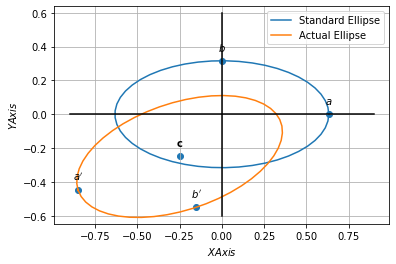
\includegraphics[width = \columnwidth]{./solutions/40/2/Ellipse.png}
\caption{Graphical representation of the ellipse}
\label{eq:solutions/15/40/2/fig:my_label}
\end{figure}

